\documentclass[10pt]{article}
\usepackage[UTF8]{ctex}

\usepackage[utf8]{inputenc} % allow utf-8 input

\usepackage{amsmath,amscd}
\usepackage{amssymb,array}
\usepackage{amsfonts,latexsym}
\usepackage{graphicx,subfig,wrapfig}
\usepackage{times}
\usepackage{psfrag,epsfig}
\usepackage{verbatim}
\usepackage{tabularx}
\usepackage[pagebackref=true,breaklinks=true,letterpaper=true,colorlinks,bookmarks=false]{hyperref}
\usepackage{cite}
\usepackage{algorithm}
\usepackage{multirow}
\usepackage{caption}
\usepackage{algorithmic}
\usepackage[amsmath,thmmarks]{ntheorem}
\usepackage{listings}
\usepackage{color}
\usepackage{bm}

\newtheorem{thm}{Theorem}
\newtheorem{mydef}{Definition}

\DeclareMathOperator*{\rank}{rank}
\DeclareMathOperator*{\trace}{trace}
\DeclareMathOperator*{\acos}{acos}
\DeclareMathOperator*{\argmax}{argmax}


\renewcommand{\algorithmicrequire}{ \textbf{Input:}}     
\renewcommand{\algorithmicensure}{ \textbf{Output:}}
\renewcommand{\mathbf}{\boldsymbol}
\newcommand{\mb}{\mathbf}
\newcommand{\matlab}[1]{\texttt{#1}}
\newcommand{\setname}[1]{\textsl{#1}}
\newcommand{\Ce}{\mathbb{C}}
\newcommand{\Ee}{\mathbb{E}}
\newcommand{\Ne}{\mathbb{N}}
\newcommand{\Se}{\mathbb{S}}
\newcommand{\norm}[2]{\left\| #1 \right\|_{#2}}

\newenvironment{mfunction}[1]{
	\noindent
	\tabularx{\linewidth}{>{\ttfamily}rX}
	\hline
	\multicolumn{2}{l}{\textbf{Function \matlab{#1}}}\\
	\hline
}{\\\endtabularx}

\newcommand{\parameters}{\multicolumn{2}{l}{\textbf{Parameters}}\\}

\newcommand{\fdescription}[1]{\multicolumn{2}{p{0.96\linewidth}}{
		
		\textbf{Description}
		
		#1}\\\hline}

\newcommand{\retvalues}{\multicolumn{2}{l}{\textbf{Returned values}}\\}
\def\0{\boldsymbol{0}}
\def\b{\boldsymbol{b}}
\def\bmu{\boldsymbol{\mu}}
\def\e{\boldsymbol{e}}
\def\u{\boldsymbol{u}}
\def\x{\boldsymbol{x}}
\def\v{\boldsymbol{v}}
\def\w{\boldsymbol{w}}
\def\N{\boldsymbol{N}}
\def\X{\boldsymbol{X}}
\def\Y{\boldsymbol{Y}}
\def\A{\boldsymbol{A}}
\def\B{\boldsymbol{B}}
\def\y{\boldsymbol{y}}
\def\cX{\mathcal{X}}
\def\transpose{\top} % Vector and Matrix Transpose

%\long\def\answer#1{{\bf ANSWER:} #1}
\long\def\answer#1{}
\newcommand{\myhat}{\widehat}
\long\def\comment#1{}
\newcommand{\eg}{{e.g.,~}}
\newcommand{\ea}{{et al.~}}
\newcommand{\ie}{{i.e.,~}}

\newcommand{\db}{{\boldsymbol{d}}}
\renewcommand{\Re}{{\mathbb{R}}}
\newcommand{\Pe}{{\mathbb{P}}}

\hyphenation{MATLAB}

\usepackage[margin=1in]{geometry}

\begin{document}
	
\title{	Numerical Optimization, 2020 Fall\\Homework $2$}
\date{Due on 14:59, Sep 24, 2020\\}
\maketitle

%%%%%--------------------

\section{线性规划标准型}
考虑如下为标准型的线性规划:
\begin{equation}\label{eq: problem1}
	\begin{aligned}
		\min_{\bm{x}}~\quad&\bm{c}^{\top}\bm{x}\\
		\textrm{s.t.}~\quad&\bm{A}\bm{x} = \bm{b}\\
		&\bm{x}\geq \bm{0},
	\end{aligned}
\end{equation}
其中~$\bm{A}\in\mathbb{R}^{m\times n}$, $\bm{c}\in\mathbb{R}^{n}$ 和 $\bm{b}\in\mathbb{R}^{m}$给定.
\begin{itemize}
	\item[$(1)$] 上述标准型~\eqref{eq: problem1}~中关于$\bm{A}$满秩 (full rank) 的假设是否合理? 请给出你判断的理由.~\textcolor{red}{[10pts]}
	
	\item[$(2)$] 在标准型里, 一个基本可行解~(basic feasible solutions)~是否与一组基 (basis)~一一对应?~\textcolor{red}{[15pts]}
\end{itemize}
\textbf{解:}
\begin{enumerate}
\item 合理。引用MIT这本教材中的定理2.5: \\
Let $P=\{x|Ax=h, x\ge O\}$ be a nonempty polyhe­dron, where A is a matrix of dimensions $m\times n$, with rows $a_1',...,a_m'$. Suppose that rank(A) = k <m and that the rows $a_{i_1}',...,a_{i_k}'$ are linearly independent. Consider the polyhedron
$$Q=\{x|a_{i_1}'x=b_{i_1},...,a_{i_k}'x=b_{i_k},x\ge0\}$$
Then Q=P.(证明思路即利用向量空间中的线性组合的性质,证明$Q\subset P,P\subset Q$)
所以在标准型下的可行域为非空的情况下,A的冗余约束对应的线性独立行可以被消去,因此行满秩的假设是合理的。下为该定理的简略证明:\\
假设$i_1=1,...i_k=k$,即A的前k行线性独立,如若不然,通过行变换即可,显然任意P中的元素均满足Q中定义的约束,因此我们可以得到$P\subset Q$。\\
其次,A中的各行均可表示为前k行的线性组合,即$a_i'=\sum_{j=1}\lambda_{ij}a_j'$.取x为P中一个元素,则有
$$b_i=a_i'x=\sum_{j=1}^k\lambda_{ij}a_j'x=\sum_{j=1}^k\lambda_{ij}b_j$$
对于Q中的任意元素y,有
$$a_i'y=\sum_{j=1}^{k}\lambda_{ij}a_j'y=\sum_{j=1}^k\lambda_{ij}b_j=b_i$$
因此$P\subset Q, Q\subset P$,于是$Q=P$.
\item 不是一一对应的。一组基对应一个基本解,只有当该非基本解非负的情况下才是一个基本可行解。例如,
	\begin{equation*}
	A=\left[
	\begin{array}{ccc}
	1 & 2 & 4 \\
	1 & 3 & 5 \\
	\end{array}
	\right], 
	b=\left[
	\begin{array}{c}
	-3 \\
	-4 \\
	\end{array}
	\right]
	\end{equation*}
	一组基
	$
	A=\left[
	\begin{array}{ccc}
	1 & 2  \\
	1 & 3  \\
	\end{array}
	\right]
	$	对应的基本解为$\left[
	\begin{array}{c}
	-1 \\
	-1 \\
	\end{array}
	\right]
	$并不是基本可行解。
\end{enumerate}



\section{基本解和基本可行解} 
考虑如下线性规划问题 (具体地, 请参考Lecture~$2$中$37$页的例~$3$)
\begin{equation}\label{eq: ex3}
	\begin{array}{c}
		\begin{aligned}
			\min~&-2 x_{1}-x_{2} \\
			\textrm { s.t. } &x_{1}+\frac{8}{3} x_{2} \leq 4, \\
			&x_{1}+x_{2} \leq 2, \\
			&2 x_{1} \leq 3, \\
			&x_{1} \geq 0, x_{2} \geq 0.
		\end{aligned}
	\end{array}
\end{equation}
请回答此问题中有多少个基本解(basic solutions), 有多少个基本可行解? 请分别写出相应的解.~\textcolor{red}{[25pts]}
\textbf{解:}
\begin{itemize}
\item 基本解9个,求解思路为联立每2个独立的积极约束确定每一个基本解,求解过程出于简洁性的考虑,在此就例举一种约束组合。
\begin{align*}
x_1+\frac{8}{3}x_2&=4\\
x_1+x_2&=2\\
\Rightarrow x_1 = \frac{4}{5}&, x_2=\frac{6}{5}
\end{align*}
将任意两个积极约束联立,我们得到求解结果: $(x_1,x_2)=(\frac{4}{5},\frac{6}{5}),(\frac{3}{2},\frac{15}{16}),(0,\frac{3}{2}),(4,0),(\frac{3}{2},\frac{1}{2}),(0,2),(2,0),(\frac{3}{2},0),(0,0)$.
\item 基本可行解5个,求解思路为,在已经求出基本解的情况下,找出满足所有约束的基本解即为基本可行解,在此例举一种基本可行解的判断
\begin{align*}
x_1 = 0,x_2&=\frac{3}{2}\\
x_1+\frac{8}{3}x_2=4&\le4\\
x_1+x_2=\frac{3}{2}&\le 2\\
2x_1=0&\le 3\\
x_1,x_2&\ge 0 \\
\Rightarrow x_1 = 0,x_2&=\frac{3}{2} \textbf{是基本可行解}
\end{align*}

对每个基本解进行同样的操作,求解结果为: $(x_1,x_2)=(\frac{4}{5},\frac{6}{5}), (0,\frac{3}{2}), (\frac{3}{2},0), (0,0),(\frac{3}{2},\frac{1}{2})$.
\end{itemize}


\section{极点}
\begin{itemize}
	\item[$1.$] 证明如下两个集合的极点一一对应.~\textcolor{red}{[12pts]}
	\begin{equation}\label{prob.Linf}
		\begin{aligned}
			S_1 &= \{\bm{x}\in\mathbb{R}^{n}\mid \bm{A}\bm{x}\leq\bm{b}, \bm{x}\geq\bm{0}\},\\
			S_2 &= \{(\bm{x},\bm{y})\in\mathbb{R}^{n}\times\mathbb{R}^{m}\mid \bm{A}\bm{x} + \bm{y} = \bm{b}, \bm{x}\geq\bm{0}, \bm{y}\geq\bm{0}\}.
		\end{aligned}
	\end{equation}
	\textbf{解:}\\
	设P和Q分别是在$R^n,R^m$中的多面体。定义ispmorphic为:if there exist affine functions f : P 􏰏→ Q and g : Q 􏰏→ P such that
	$$x=g(f(x)),\forall x \in P,\quad\quad y=f(g(x)),\forall y\in Q$$
	\begin{itemize}
	\item 首先,先证明如果P和Q是isomorphic,那么他们的极点是一一对应的。假设$x^\star$是P的一个极点,设$y^\star = f(x^\star)$。因为$x^\star$是P的一个极点,所以存在一个向量$c\in R^n$使得
	$$c^Tx<c^Tx,\quad\quad\forall x\in P,x\neq x^\star$$
	那么对于任意$y\in Q,y\neq y^\star$,我们有
	$$f(g(y))=y\neq y^\star =f(x^\star) \Rightarrow g(y)\neq x^\star$$
	因此
	$$c^Tg(y)\le c^Tg(y^\star),\qquad\forall y\in Q, y\neq y^\star$$
	令仿射函数g有$g(y)=By+d$,其中B是$n\times m$的矩阵,$d\in R^n$.于是我们有
	$$(B^Tc)^Ty<(B^Tc)^Ty\star,\qquad \forall y \in Q,y\neq y^\star$$
	如果$y^\star$不是Q的极点,那么我们可以得到$y^\star=\alpha y_1+(1-\alpha)y_2$,其中$y_1,y_2\in Q,y_1\neq y^\star,y_2\neq y^\star,\alpha\in(0,1)$,所以
	$$(B^Tc)^Ty^\star =\alpha(B^Tc)^Ty_1+(1-\alpha)(B^Tc)^Ty_2<(B^Tc)^Ty^\star$$
	这显然与已知矛盾,所以$y^\star$也是Q的极点。相反地,如果$y^\star$是Q的极点的话,那么通过相同的论证,我们可以证明$x^\star$也是P的极点。因此,如果P和Q是isomorphic,那么他们的极点是一一对应的。
	\item 接着我们证明$S_1$和$S_2$是isomorphic。令f和g分别为
	\begin{align*}
	f(x)=(x,b-Ax),\qquad\forall x\in S_1,\\
	g(x,z)=x,\qquad \forall(x,z)\in S_2.
	\end{align*}
	显然,f和g均为仿射函数:
	\begin{align*}
	f(x)\in S_2,\qquad g(f(x))&=x, \qquad\forall x\in S_1,\\
	g(x,z)\in S_1,\qquad f(g(x,z))&=(x,z), \qquad\forall (x,z)\in S_2
	\end{align*}
		
	因此,$S_1$和$S_2$是isomorphic。综上对于$S_1,S_2$,由于他们是isomorphic,所以他们的极点一一对应。
	\end{itemize}
	\item[$2.$]
	如图~\ref{fig: linear program}~所示, 请回答
	\begin{itemize}
		\item[$(1)$] 集合$P = \{\bm{x}\in\mathbb{R}^{2}\mid 0\leq x_1\leq 1\}$有极点吗?~\textcolor{red}{[3pts]}
		
		\item[$(2)$] 它的标准型是什么?~\textcolor{red}{[5pts]}
		
		\item[$(3)$] 它的标准型有极点吗? 若有, 则给出一个极点, 并解释为什么是极点.~\textcolor{red}{[5pts]}
	\end{itemize}
	\textbf{解:}
	\begin{enumerate}
	\item 没有极点,因为可行域包含了一条直线。
	\item 
	\begin{equation*}\label{eq: ex3}
	\begin{array}{c}
		\begin{aligned}
			\min~& \text{constant k} \\
			\textrm { s.t. } & x_1 + s =1, \\
			&x_1,x_2^+,x_2^-,s\ge0 \\
		\end{aligned}
	\end{array}
	\end{equation*}
	\item 有极点。我们先求解基本解,通过联立四个线性独立的积极约束,例如$(x_1+s=1,x_1=0,x_2^+=0,x_2^-=0),(x_1+s=1,x_2^+=0,x_2^-=0,s=0)$。然后取标准型中的非负基本解即基本可行解,根据基本可行解与极点的等价定理,我们即可找到极点:$(x_1,x_2^+,x_2^-,s)=(1,0,0,0),(0,0,0,1)$。因为所求的极点为基本可行解,因此我们能保证极点的正确性。

	\end{enumerate}
\end{itemize}
\begin{figure}[htbp]
	\centering
	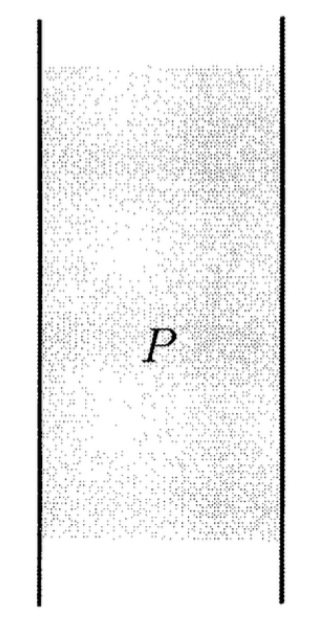
\includegraphics[width=1in]{lp.jpg}
	\caption{集合P}
	\label{fig: linear program}
\end{figure}



\section{AMPL实现}
考虑如下~Haverly pooling~问题, 如图~\ref{fig: Haverly}~示, 请使用AMPL实现并求解.
\begin{figure}[htbp]
	\centering
	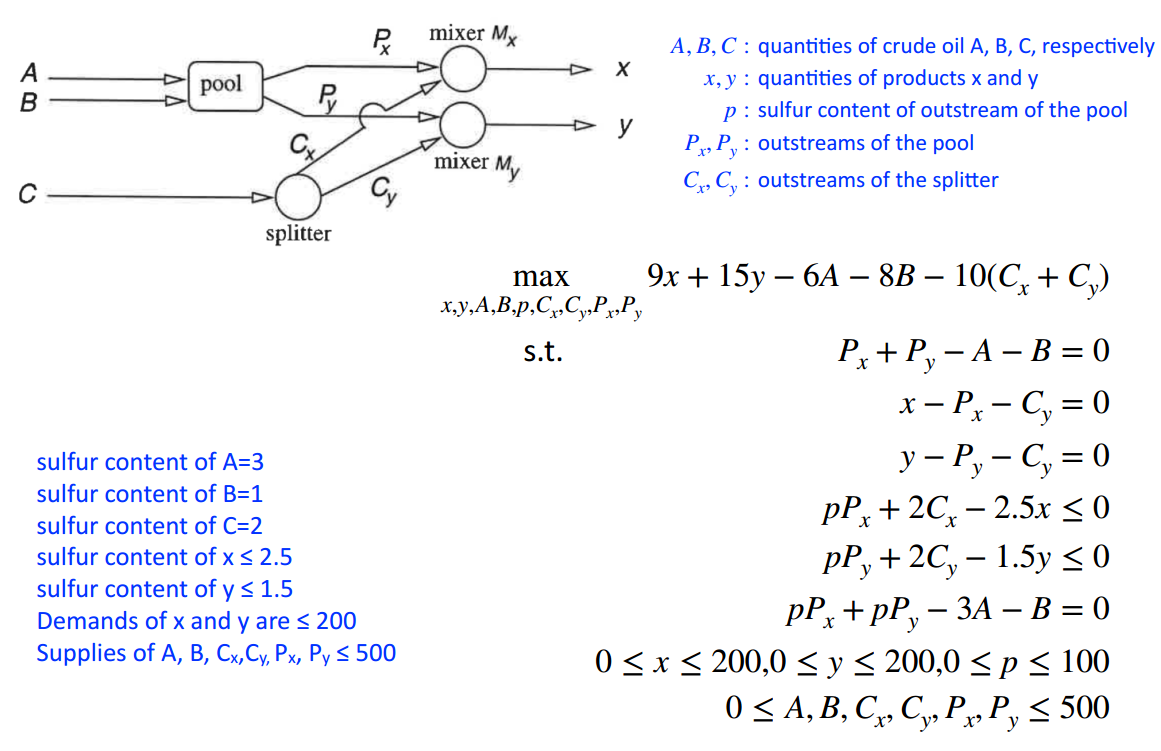
\includegraphics[width=4in]{Haverly pooling.jpg}
	\caption{Example: Haverly Pooling Problem.}
	\label{fig: Haverly}
\end{figure}
(注意: 使用AMPL solver或者NEOS solver均可. 另外, 请在提交的作业中注明使用的求解器类型, 把求解结果呈现出来 (截图附在PDF文件即可), 并把源代码一起提交. 提交的作业请打包为.zip文件, 包含你的PDF以及源码.)~\textcolor{red}{[25pts]}\\
\textbf{解:}题目中第二个约束有错误,我将$C_y$改成了$C_x$. 求解器的类型是非线性求解器Baron,求解结果为1800.
\begin{figure}[!h]
	\centering
	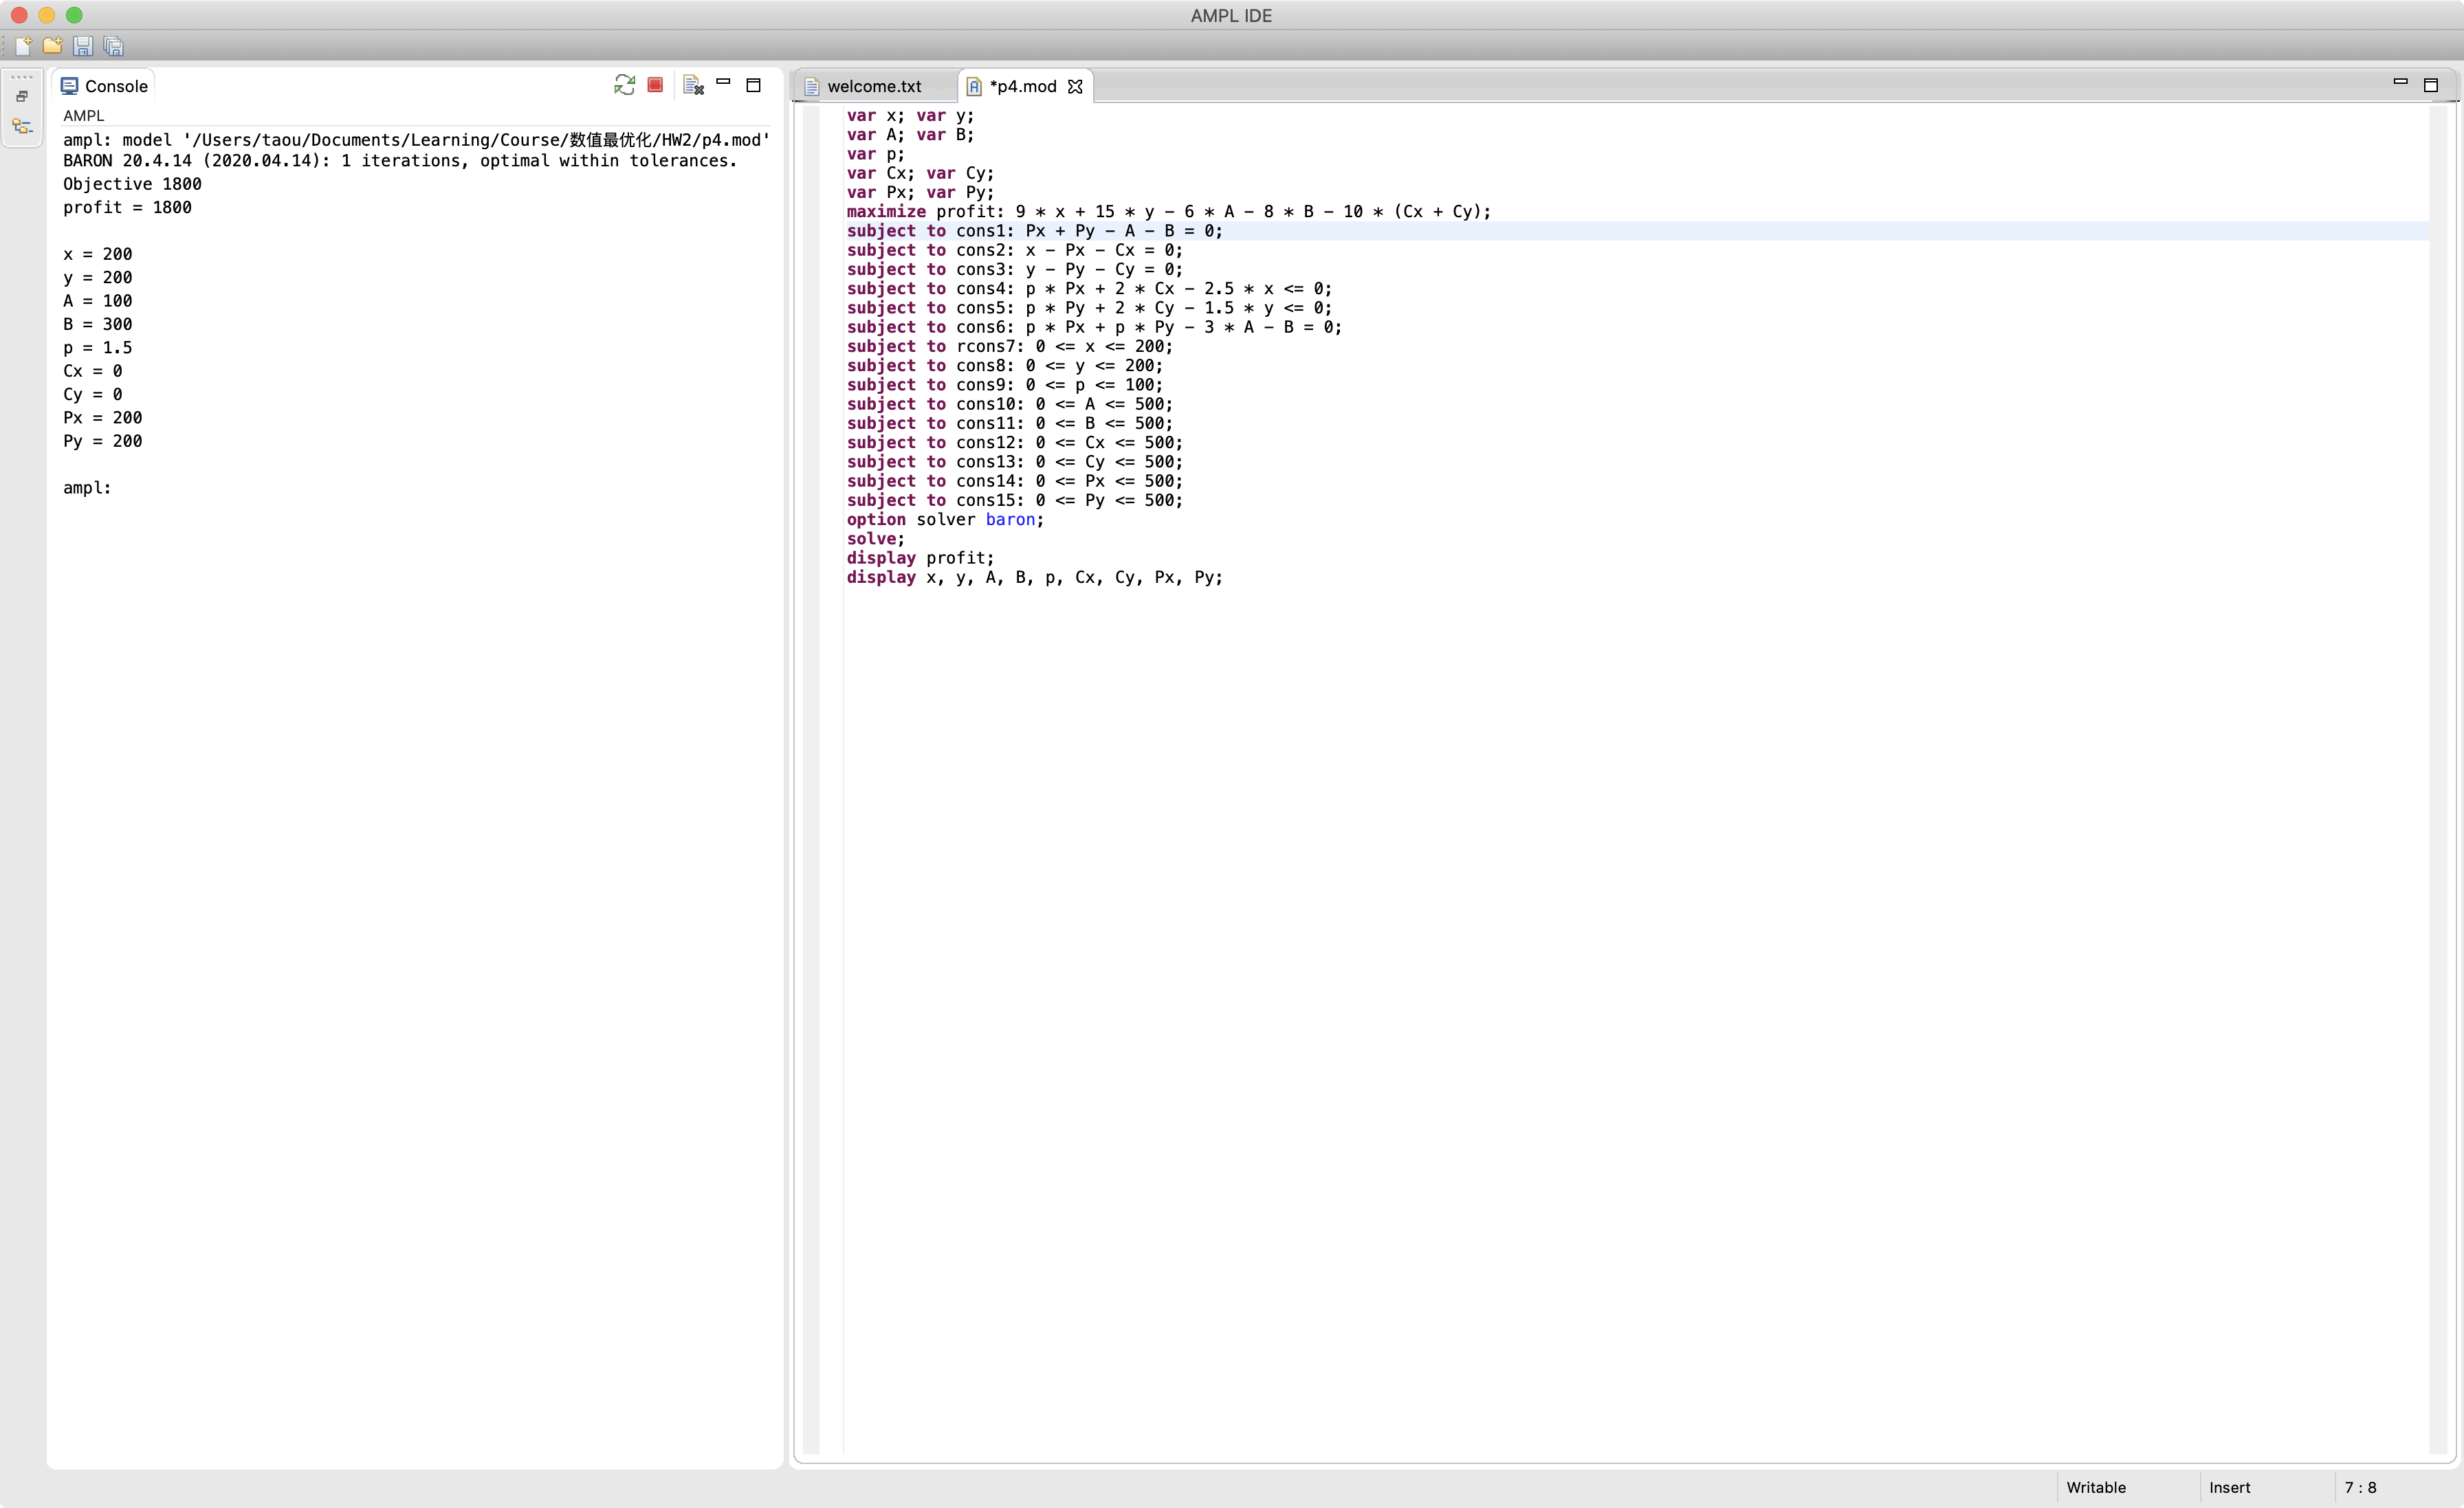
\includegraphics[width=6in]{p4.png}
	\caption{集合P}
	\label{fig: linear program}
\end{figure}
\end{document} 